\chapter*{Introduction}
\addcontentsline{toc}{chapter}{Introduction}
One of the big unsolved problems of modern physics is constructing the quantum computer. The implications here are mainly to so-called \emph{adiabatic quantum computers}, where the solution to some mathematical problem is substituted for finding the wavefunction corresponding to the global energy minima of some system. This system usually consists of coupled qubits\footnote{As qubits one might use for example quantum dots \citep{dots} or Josephson junctions \citep{josephson}.}. The energy minimum can be found by numerous measurements of the specific superposition of qubits. The preparation of such a state in superposition is a complicated process, and one method of achieving it is so-called \emph{quantum annealing}\footnote{The name comes from the resemblance to annealing in metallurgy.}. Annealing is the process of changing the state from some simple \emph{initial state} to the required state in superposition (\emph{final state}). The initial state is typically chosen to be the ground state of some easily preparable configuration, such as \emph{all spins up}. The change in states is called \emph{quantum state transport} or \emph{quantum state driving}.

The point of interest of this thesis is the quantum state driving. This driving usually needs to be performed \emph{adiabatically}, i.e., without excitation of the system. The probability that the state will remain in a ground state during such transport is called \emph{fidelity}. For an illustration of this problem, see Fig. \ref{fig:introDriving}, where two scenarios are drawn. In the first case, the state moves adiabatically (fidelity is one). In the second, the state excites in the small energy gap area, which in the case of quantum computers devaluates the experiment.

\begin{figure}[H]
    \centering
    \begin{tikzpicture}
        \node[] at (0,0) {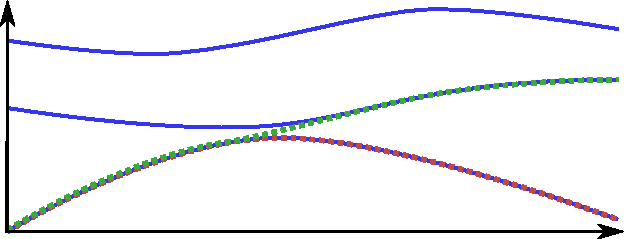
\includegraphics[width=0.6\textwidth]{../img/introDriving.pdf}};
        \node[] at (-4.5,1.6) {$\blue E$};
        \node[] at (4.6,-1.55) {$t$};
    \end{tikzpicture}
\caption{Visualization of the \redd{state adiabatic transport} compared to \greenn{transport with excitation} in a system with time varying \bluee{energy eigenstates}.}
    \label{fig:introDriving}
\end{figure}

The whole problem of state preparation can be formulated more generally. From the mathematical point of view, in the example above, we have \emph{parameter driven Hamiltonian} $\HH(\llambda)$ between qubits (omitting the thermal basis of the environment and other effects), which depends on some vector $\llambda$ from \emph{parameter space}. Change in the driving parameter (for example, the orientation of a magnetic field or strength of qubit coupling) influences the qubits and \emph{drives} them to some final state in superposition.

The question of interest is: “How to achieve the better \emph{final fidelity}, meaning \emph{how to prepare the final ground state with the higher probability}?” During the driving, one might add some energy to the qubit, which leads to its excitation and possibly destroys the superposition. Many methods can improve this. From the theory of \emph{quantum state driving} three methods are emphasized here — \emph{adiabatic driving}, \emph{counter-diabatic driving}, or \emph{choosing better driving path}. Adiabatic driving can be performed by infinitely slow drivings, making it unsuitable for practical applications. Counter-diabatic driving requires adding another element to the Hamiltonian, which leads to \emph{unit fidelity protocols} (the system does not excite), making it a good candidate for practical applications. Finding a better driving path can be combined with all other methods and means that different paths in parameter space lead to different fidelity. Because energy spectra influence these trajectories, one might be interested in the \emph{quantum state manifolds}. These are especially important for some drivings, such as driving using small \emph{quenches} (quick, but small changes in driving parameter), or close-adiabatic driving, where the fidelity is almost one.

Before moving to the theory of quantum state driving, the basics of differential geometry are presented in Chapter \ref{chap:mathIntro}. It does not serve the full theory, only some basic intuition is built, and useful definitions are provided here. The theory of quantum driving itself is described in Chapter \ref{chap:driving}. First the geometrical space is constructed, then the concept of \emph{quantum state driving}, \emph{fidelity} and \emph{metric tensor} are introduced.
The driving methods are described in Chapter \ref{chap:typesOfDriving}. Especially \emph{counter-diabatic}, \emph{adiabatic} and \emph{close-adiabatic} drivings are introduced, along with reformulation of theorems about fidelity. Special importance is played by the \emph{ground state manifold} and geodesics, for which some applications are proposed.

The basic phenomena of quantum state driving are demonstrated on a simple two-level system is analyzed in Chapter \ref{chap:twoLevelSystem}. Driving fidelity and energy variance are calculated for two special drivings — \emph{linear} and \emph{geodesic}. Finally, the more convoluted Lipkin-Meshkov-Glick model is analyzed in Chapter \ref{chap:lipkin}. The analysis is first performed in specific dimensions, from which some general formulas in arbitrary dimensions are derived. The focus is mainly on the ground state manifold and its geometrical structures. This can help to understand drivings with a unit or almost unit fidelity.